\graphicspath{{exp_design/fig/}}
{
\tikzset{external/figure name/.add={exp_design/}{}}

\chapter{Experimental design} \label{chap:exp_design}

    \paragraph
    As discussed in the literature study in Chapter~\ref{chap:lit_study}, experimental data is a valuable part of any work involving multirotors control.
    This chapter will provide an overview of the hardware, software, \gls{HITL} simulations, and practical methodology used in this work.

    \FloatBarrier\section{Hardware components}

        \paragraph
        The main hardware components in this work include a multirotor vehicle, a payload angle sensor, and an \gls{OBC}.
        These components are coupled together into the final multirotor system which will be used for practical flights.

        \FloatBarrier\subsection{Multirotor}

            \begin{figure}[ht]
                \centering
                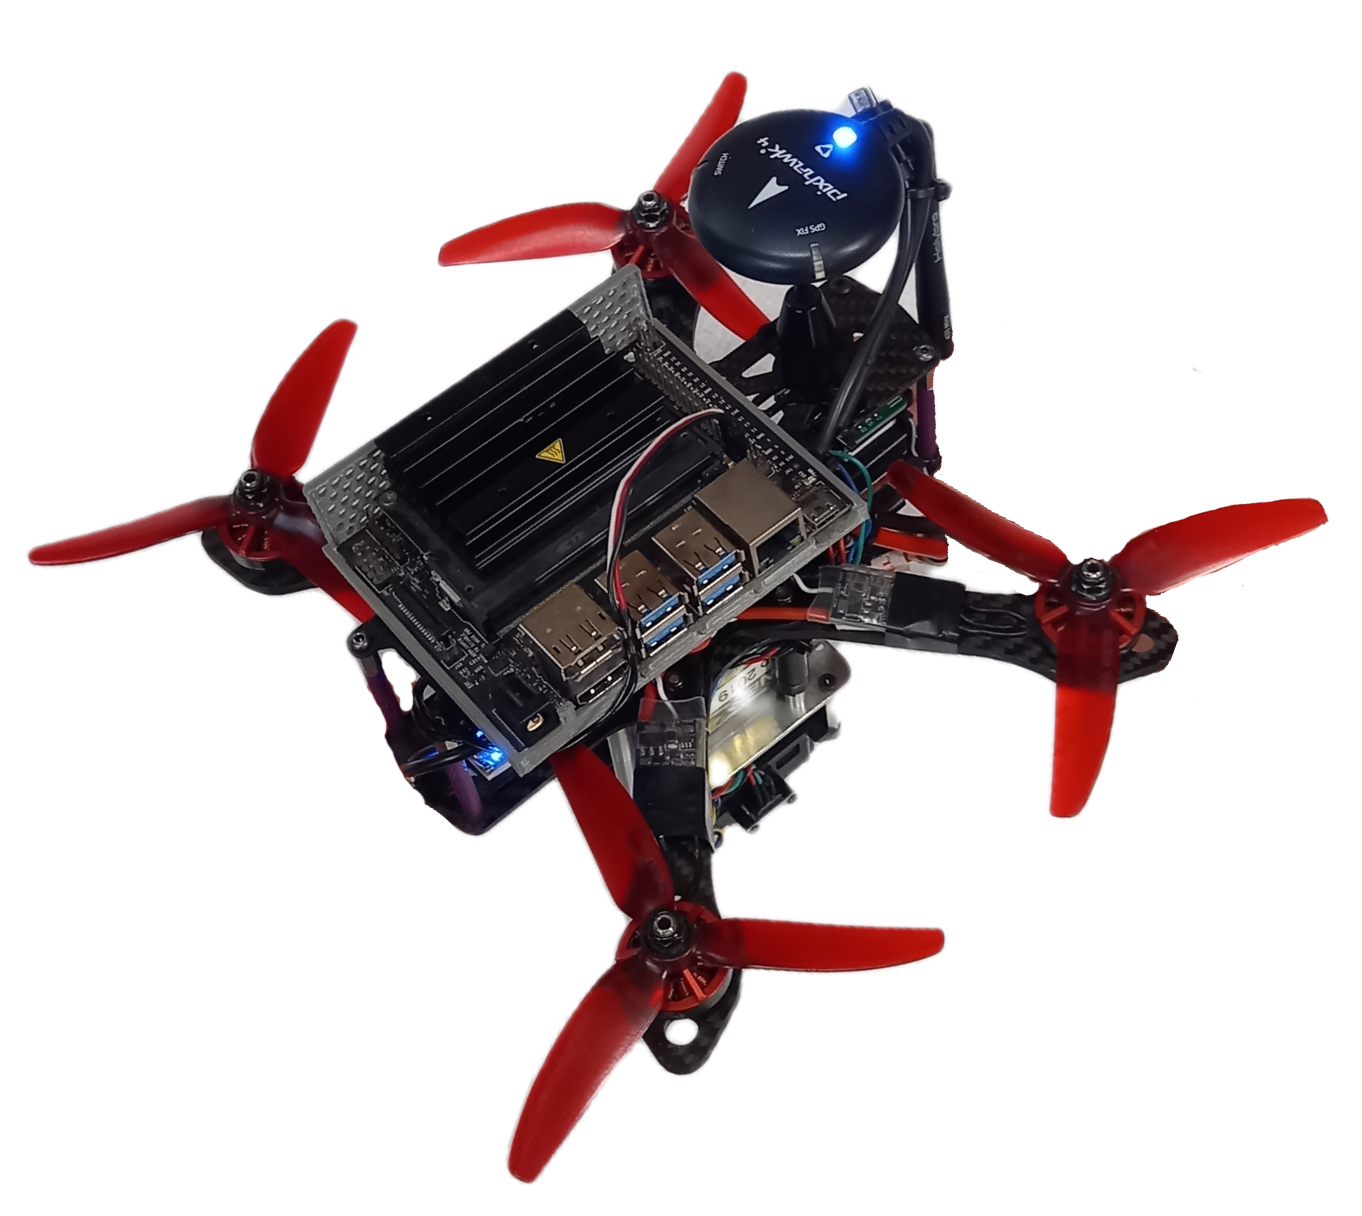
\includegraphics[width=0.5\linewidth]{exp_design/fig/honeybee}
                \caption{Honeybee multirotor equipped with a \gls{OBC} and payload angle sensor}
                \label{fig:honeybee}
            \end{figure}

            \paragraph
            The multirotor used in this work is a custom-built, lightweight multirotor named \emph{Honeybee}.
            This vehicle was developed in the \gls{ESL} at Stellenbosch University \cite{Grobler2020}.
            Figure~\ref{fig:honeybee} shows a photo of Honeybee equipped with an \gls{OBC} and payload angle sensor.
            
            \paragraph
            The physical parameters of this multirotor are summarised in Table~\ref{tbl:honeybee_specs}.
            Note that the mass and inertial parameters include the \gls{OBC} and payload angle sensor.
            The thrust profile of each motor is given by the third-order polynomial mapping the input \gls{PWM} signal, $x$, to the thrust output, $T_m$ \cite{Grobler2020}:
            \begin{equation}
                T_m(x) = -3.508 \cdot 10^{-9} x^3 + 1.627 \cdot 10^{-5} x^2 - 0.0172 x + 4.528
            \end{equation}

            \begin{table}[!h]
                \renewcommand{\arraystretch}{1.1}
                \centering
                \caption{Physical parameters of Honeybee.}
                \begin{tabularx}{0.85\linewidth}{@{}lll@{}}
                    \toprule
                    \textbf{Description} & \textbf{Parameter} & \textbf{Value} \\
                    \midrule
                    Mass                        & $m_Q$     & 0.952~kg \\
                    Motor distance              & $d$       & 0.11~m \\
                    Virtual yaw moment arm      & $R_N$     & $7.997 \cdot 10^{-3}$~m \\
                    Motor time constant         & $\tau$    & 15~ms \\
                    Mass moment of inertia about $\bm{\bar{x}}_\mathcal{B}$       & $I_{xx}$      & $2.00 \cdot 10^{-3}$~kg$\cdot$m$^2$ \\
                    Mass moment of inertia about $\bm{\bar{y}}_\mathcal{B}$       & $I_{yy}$      & $1.32 \cdot 10^{-3}$~kg$\cdot$m$^2$ \\
                    Mass moment of inertia about $\bm{\bar{z}}_\mathcal{B}$       & $I_{zz}$      & $3.35 \cdot 10^{-3}$~kg$\cdot$m$^2$ \\
                    Aerodynamic drag coefficient in $\bm{\bar{x}}_\mathcal{B}$    & $C_{Q_X}$     & 0.096~m$^2$ \\	
                    Aerodynamic drag coefficient in $\bm{\bar{y}}_\mathcal{B}$    & $C_{Q_Y}$     & 0.096~m$^2$ \\	
                    Aerodynamic drag coefficient in $\bm{\bar{z}}_\mathcal{B}$    & $C_{Q_Z}$     & 0.256~m$^2$ \\	
                    \bottomrule
                \end{tabularx}
                \label{tbl:honeybee_specs}
            \end{table}
        
            \paragraph
            The \gls{FC} implemented on Honeybee is a \emph{Pixhawk 4 mini} shown in Figure~\ref{fig:pixhawk}.
            This board includes internal \gls{IMU}, magnetometer, and barometer sensors and is connected to an external \gls{GPS} sensor and an additional magnetometer.
            Furthermore, an \gls{RC} receiver is used to communicate with a radio transmitter for manual pilot control.
            A telemetry radio module is used for communication with a ground control station.
            The \gls{OBC} and external payload angle sensors are also connected to the \gls{FC}.

            \begin{figure}[ht]
                \centering
                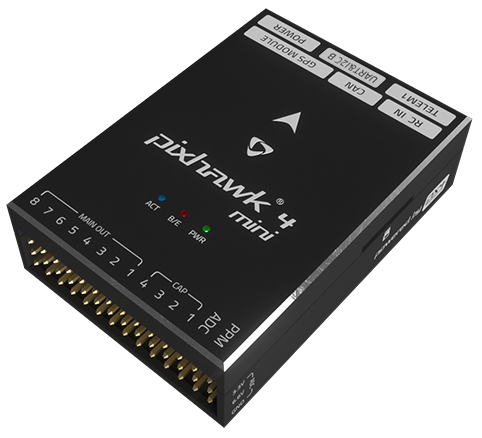
\includegraphics[width=0.3\linewidth]{exp_design/fig/pixhawk}
                \caption{Photo of a Pixhawk 4 mini \gls{FC} \cite{PX4userguide}}
                \label{fig:pixhawk}
            \end{figure}
            
        \FloatBarrier\subsection{Payload angle sensor}

            \paragraph
            A sensor is required to measure the payload state as Euler angles about the $\bm{\bar{x}}_\mathcal{B}$ and $\bm{\bar{y}}_\mathcal{B}$ axes.
            Figure~\ref{fig:payload_state_sensor} shows a customised sensor attached to the Honeybee airframe for this purpose.
            
            \begin{figure}[ht]
                \centering
                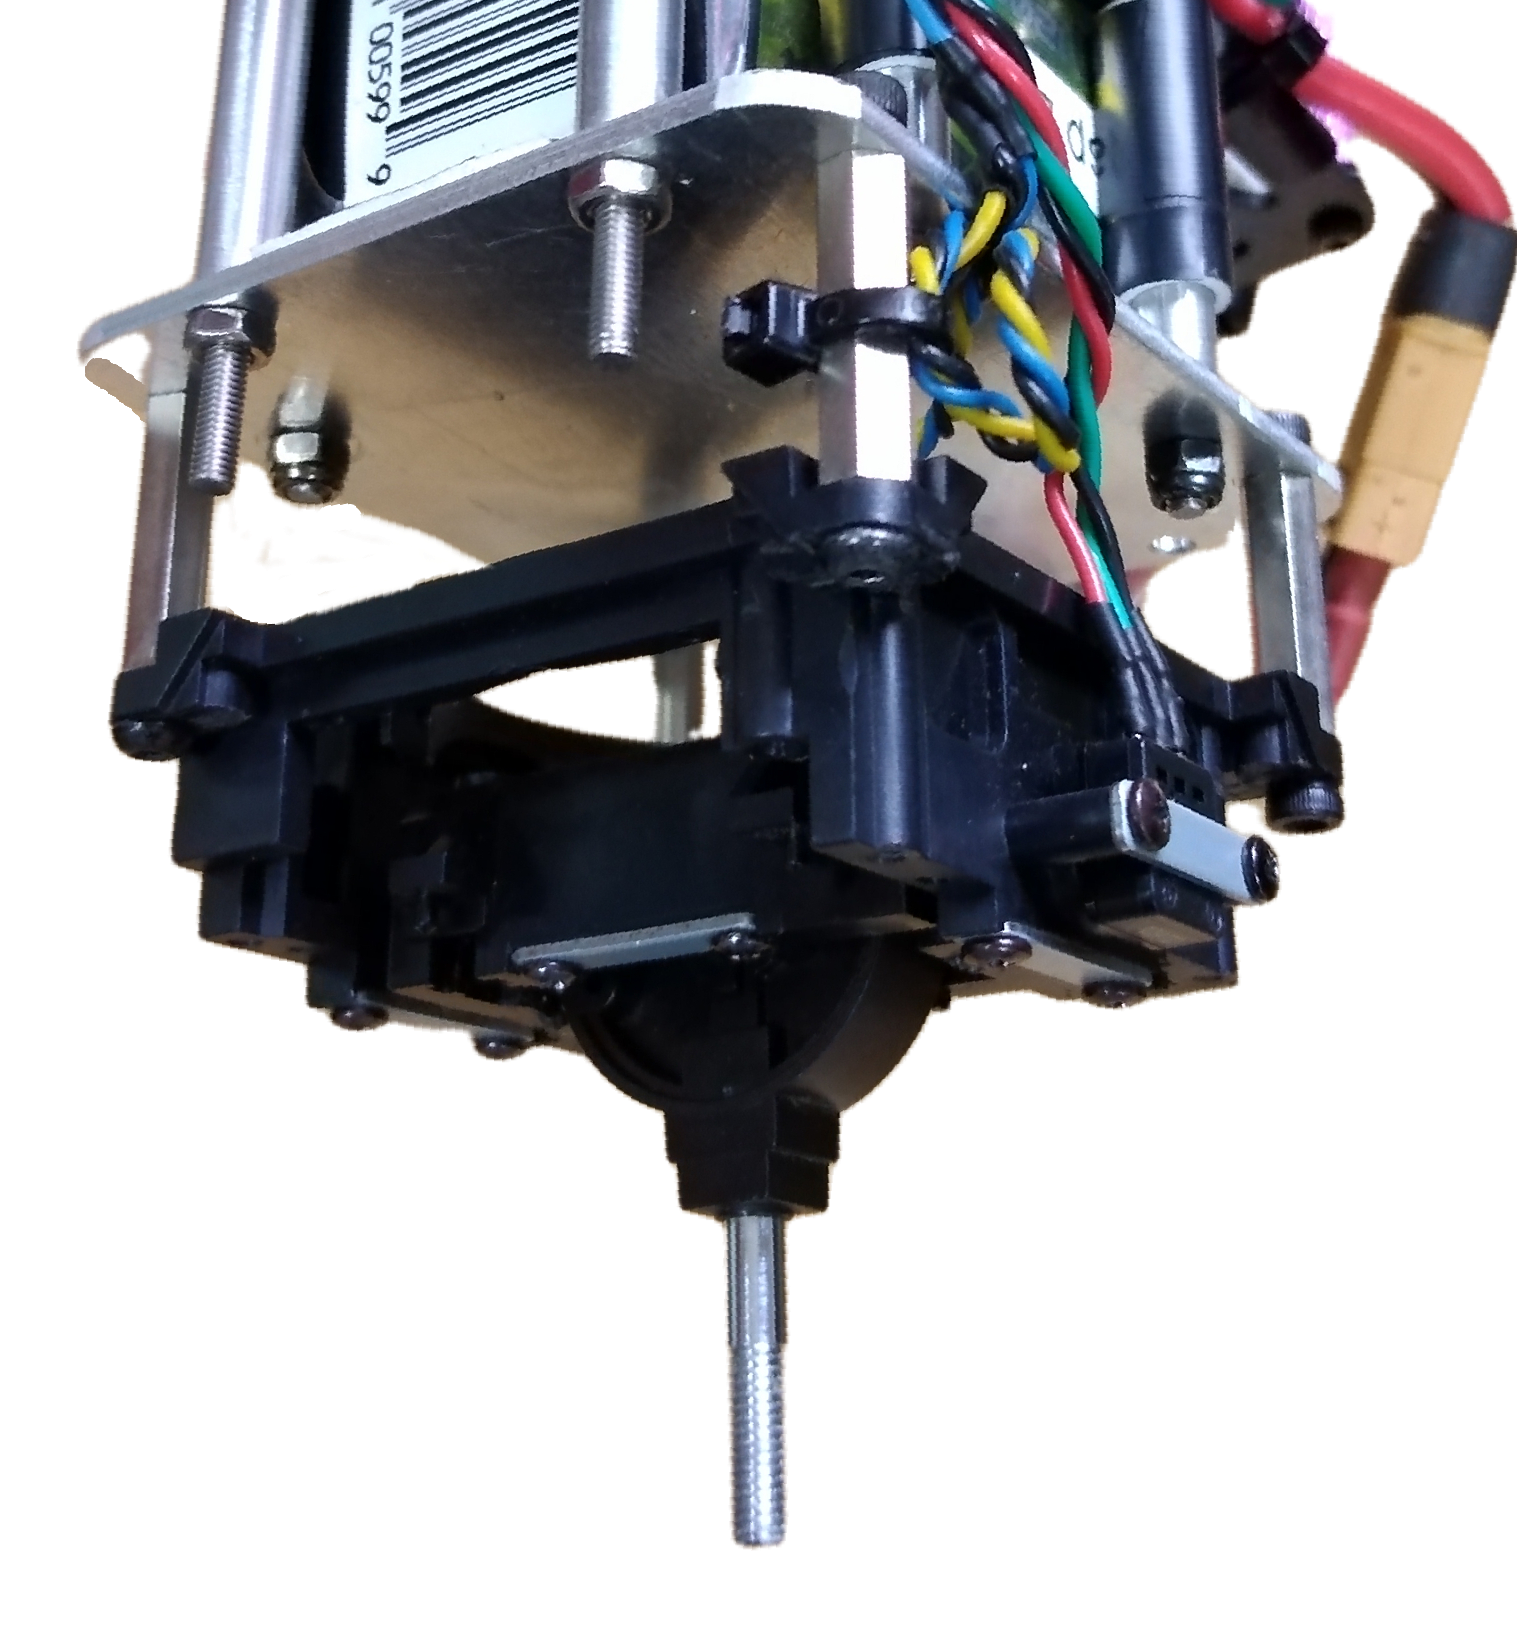
\includegraphics[width=0.3\linewidth]{exp_design/fig/payload_state_sensor}
                \caption{Payload angle sensor with linear potentiometers}
                \label{fig:payload_state_sensor}
            \end{figure}

            \paragraph
            This sensor was constructed from a two-axis joy-stick and two linear potentiometers.
            Each potentiometer is implemented as a voltage divider and attached to an \gls{ADC} channel on the \gls{FC}. 
            Experimental data was used to map the \gls{ADC} reading to an angle measurement with a best-fit straight line function.
            A cable can therefore be attached to this device to transport a suspended payload and measure the payload swing angles during flight.

        \FloatBarrier\subsection{On-Board Computer}

            \paragraph
            An \gls{OBC}, also called a companion computer, is used to run intensive computational processes that cannot be handled by the \gls{FC}.
            A NVIDIA\textsuperscript{\textregistered} Jetson Nano\texttrademark, which is shown in Figure~\ref{fig:jetson}, is used as the \gls{OBC} for Honeybee.
            This has 4GB memory and a quad-core processor which runs at 1.43 GHz.
            The \gls{OBC} is connected to a serial port on the \gls{FC} for communication.

            \begin{figure}[ht]
                \centering
                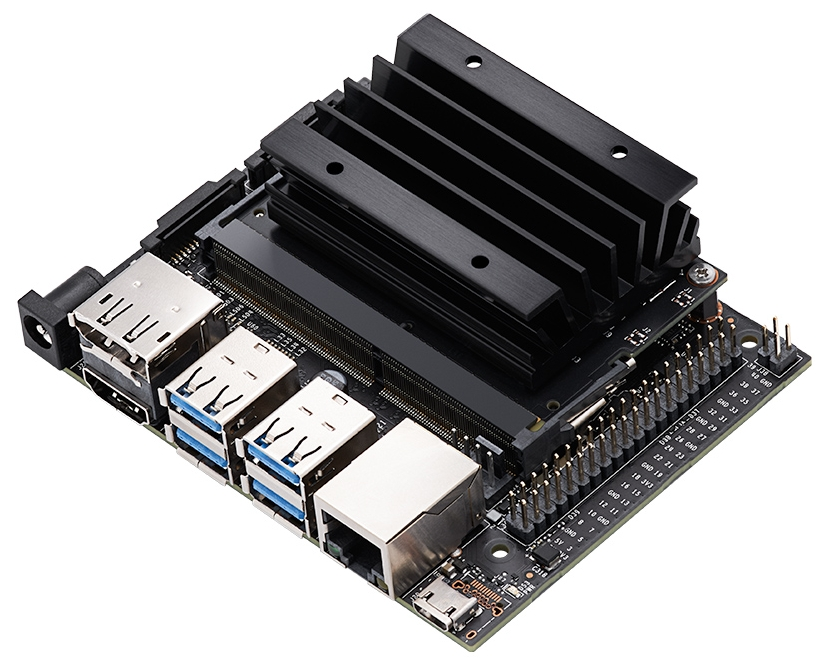
\includegraphics[width=0.3\linewidth]{exp_design/fig/jetson}
                \caption{NVIDIA\textsuperscript{\textregistered} Jetson Nano\texttrademark~\cite{NVIDIA} used as a \gls{OBC}}
                \label{fig:jetson}
            \end{figure}
            
    \FloatBarrier\section{Software Toolchain}

        \paragraph
        The software toolchain used with Honeybee includes PX4, QGroundControl, \gls{ROS}, and Gazebo simulator.
        This toolchain and was also implemented and described well by \citet{Erasmus2020}, \citet{Slabber2020}, and \citet{Grobler2020}.
        A brief overview of the software toolchain is provided here.
        % Simulink\texttrademark~was also used to generate standalone \gls{ROS} nodes which runs on the \gls{OBC}.

        \subsection{PX4}

            \paragraph
            PX4 is an open-source flight-stack that focuses on autonomous \glspl{UAV} \cite{Meier2015} and is used in research and industrial applications.
            \gls{SITL} and \gls{HITL} simulations are supported by PX4, which is helpful for research and development.
            
        \subsection{QGroundControl}
        
            \paragraph
            \gls{QGC} is the recommended ground station software for PX4 systems \cite{PX4userguide}.
            A ground station computer running \gls{QGC} can be used to monitor and control a PX4 vehicle.
            \gls{QGC} communicates with PX4 via the MAVLink protocol over a telemetry connection during practical flights.
            During \gls{SITL} simulations, \gls{QGC} connects to PX4 over a local \gls{UDP} connection.
            \gls{QGC} is also an open-source product.
            
        \subsection{Gazebo simulator}

            \paragraph
            Gazebo is an open-source graphical-based physics simulator used for robotics.
            This is the recommended simulator in the PX4 development toolchain and is capable of both \gls{SITL} and \gls{HITL} simulations \cite{PX4userguide}.
            The PX4 flight-stack includes multirotor models developed for Gazebo which include realistic sensor plugins.
            These plugins apply sensor noise, drift and bias which replicates the actual sensors used on Pixhawk boards.
            The physical parameters of these models were changed to match Honeybee and a suspended payload was added to the model as shown in Figure~\ref{fig:gazebo_honeybee}.

            \begin{figure}[ht]
                \centering
                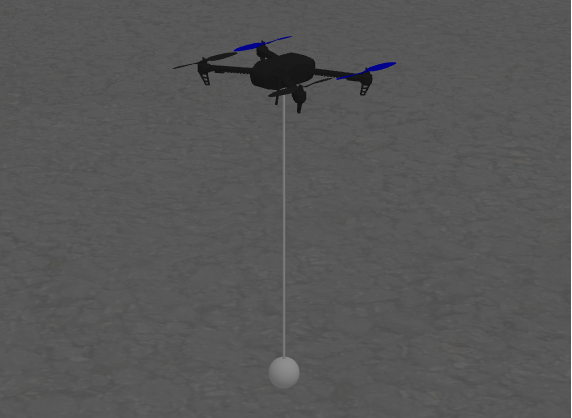
\includegraphics[width=0.6\linewidth]{exp_design/fig/gazebo_honeybee}
                \caption{Model of Honeybee in the Gazebo simulator}
                \label{fig:gazebo_honeybee}
            \end{figure}

        \subsection{Robot Operating System}

            \paragraph
            \gls{ROS} is a communication framework with a set of tools used for robotics and control applications \cite{Quigley2009}. 
            \gls{ROS} is also open-source and is supported by PX4.
            In this framework, executables are called \gls{ROS} nodes and these nodes interact with each with a publish-subscribe architecture.
            A \gls{ROS} node can publish messages to a topic, and a different node can subscribe to that topic to read those messages.

            \paragraph
            MAVROS is an open-source \gls{ROS} package that provides a bridge between \gls{ROS} and PX4 through the MAVLink protocol.
            % \gls{QGC} and Gazebo also communicate with PX4 through MAVLink.
            A MAVROS node receives MAVLink messages from PX4 and converts this to published \gls{ROS} topics for other \gls{ROS} nodes to access.
            The MAVROS node also subscribes to other topics to receive \gls{ROS} messages and send this data to PX4. 

            \begin{figure}[!htbp]
                \centering
                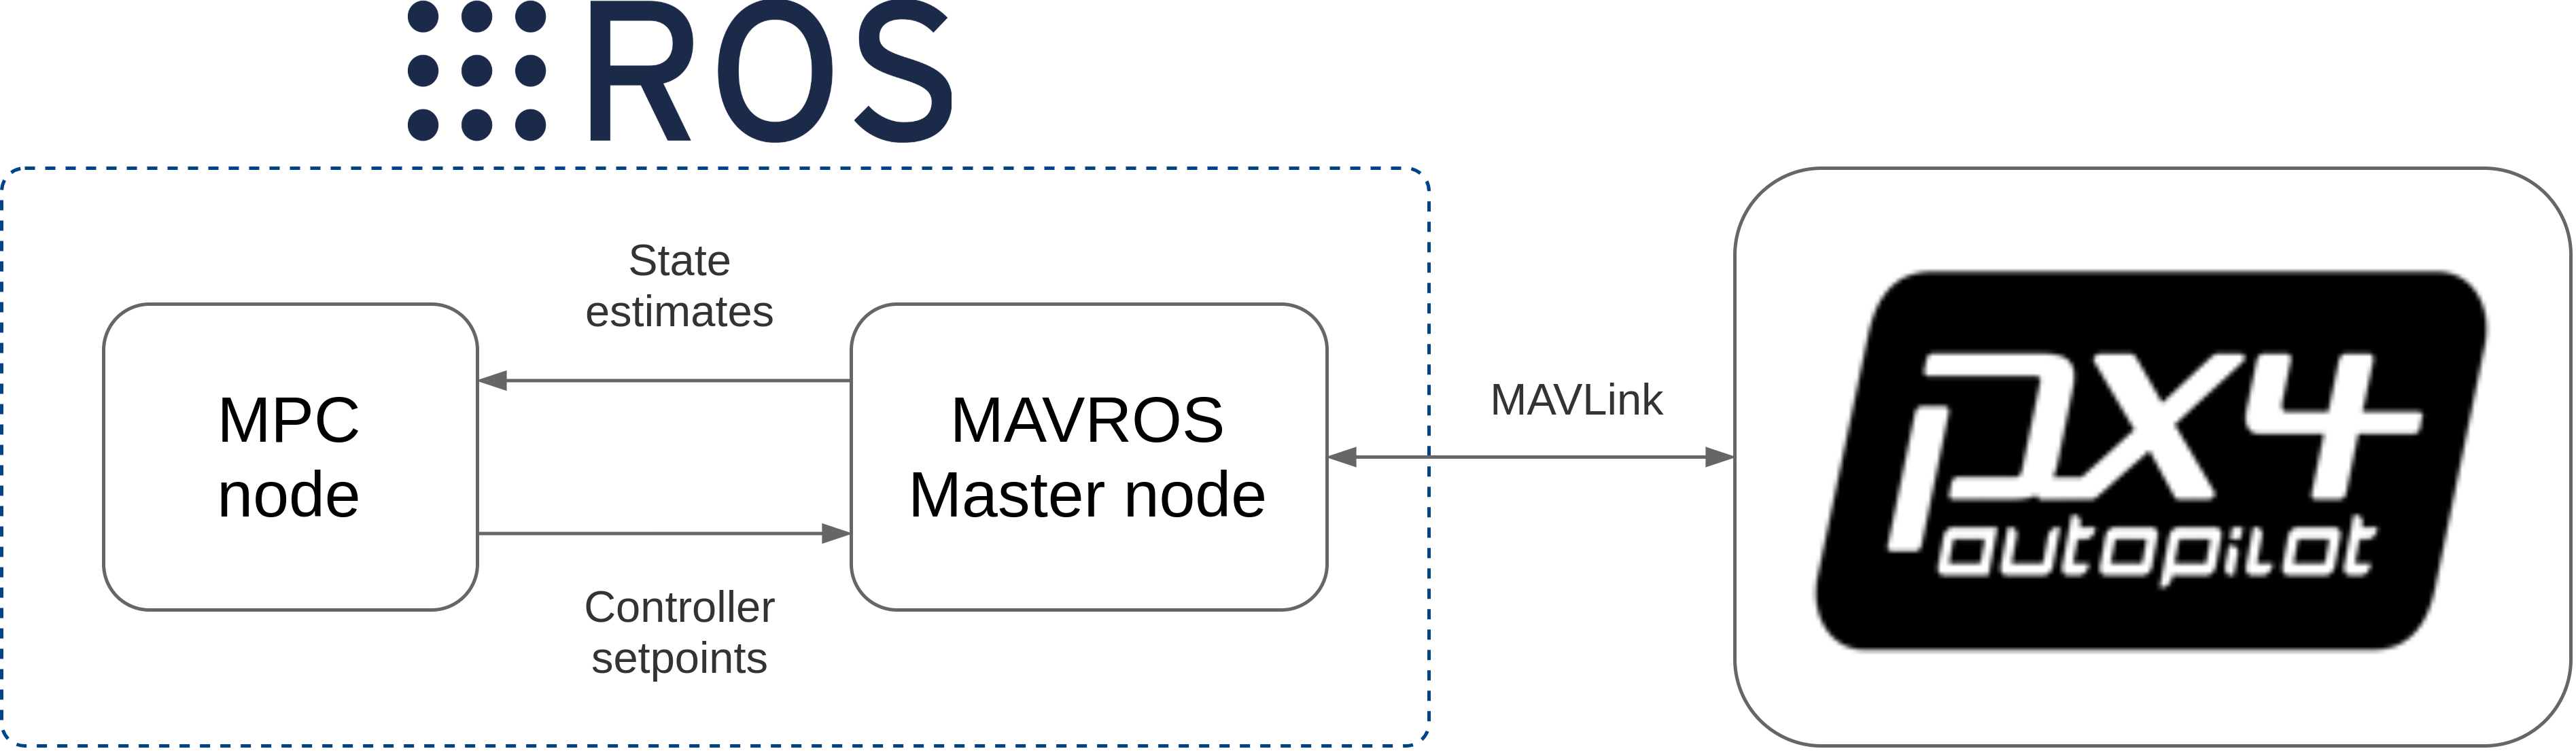
\includegraphics[width=0.9\linewidth]{exp_design/fig/MAVROS}
                \caption{Communication between \gls{ROS}, flight-stack, simulator, and ground station~\cite{Grobler2020}}
                \label{fig:MAVROS}
            \end{figure}

            \paragraph
            Simulink\texttrademark~was used to convert the \gls{MPC} controller developed in Section~\ref{sec:mpc} to C\texttt{++} code and generate a standalone \gls{ROS} node.
            Figure~\ref{fig:MAVROS} illustrates how the \gls{MPC} node is used as an offboard controller with PX4 and MAVROS.
            A MAVROS Master node receives data, including state estimates, from PX4 through MAVLink communication. 
            This data is published by MAVROS to various \gls{ROS} topics.
            State estimate data is received by the \gls{MPC} node by subscribing to the appropriate MAVROS topic.
            After the \gls{MPC} node calculates the next controller decision, it publishes the controller setpoint data to a MAVROS topic.
            The MAVROS node then sends it to PX4 via MAVLink.

    \FloatBarrier\section{Hardware-in-the-Loop simulations} \label{sec:exp_design_hitl}

        \paragraph
        In \gls{HITL} simulations, the simulator mimics the sensor outputs, but the PX4 firmware and the accompanying software runs on the designated hardware.
        Figure~\ref{fig:HITL} illustrates how the different software and hardware components interlink for \gls{HITL} simulations.
        
        \paragraph
        \gls{QGC} runs on the desktop computer and communicates with the Gazebo simulator with MAVlink messages over a local \gls{UDP} connection.
        The Gazebo simulator also runs on the desktop computer and simulates the Honeybee multirotor.
        The simulator mimics the multirotor sensor values and sends them to PX4 with MAVlink messages over a \gls{USB} connection. 
        
        \paragraph
        The PX4 firmware runs on the \gls{FC} board.
        Based on the received sensors values, the PX4 controllers determine \gls{PWM} actuator commands which are communicated back to Gazebo.
        The \gls{OBC} runs the \gls{MPC} and MAVROS nodes which send and receive MAVLink messages over a serial port connection to the \gls{FC}.

        \begin{figure}[ht]
            \centering
            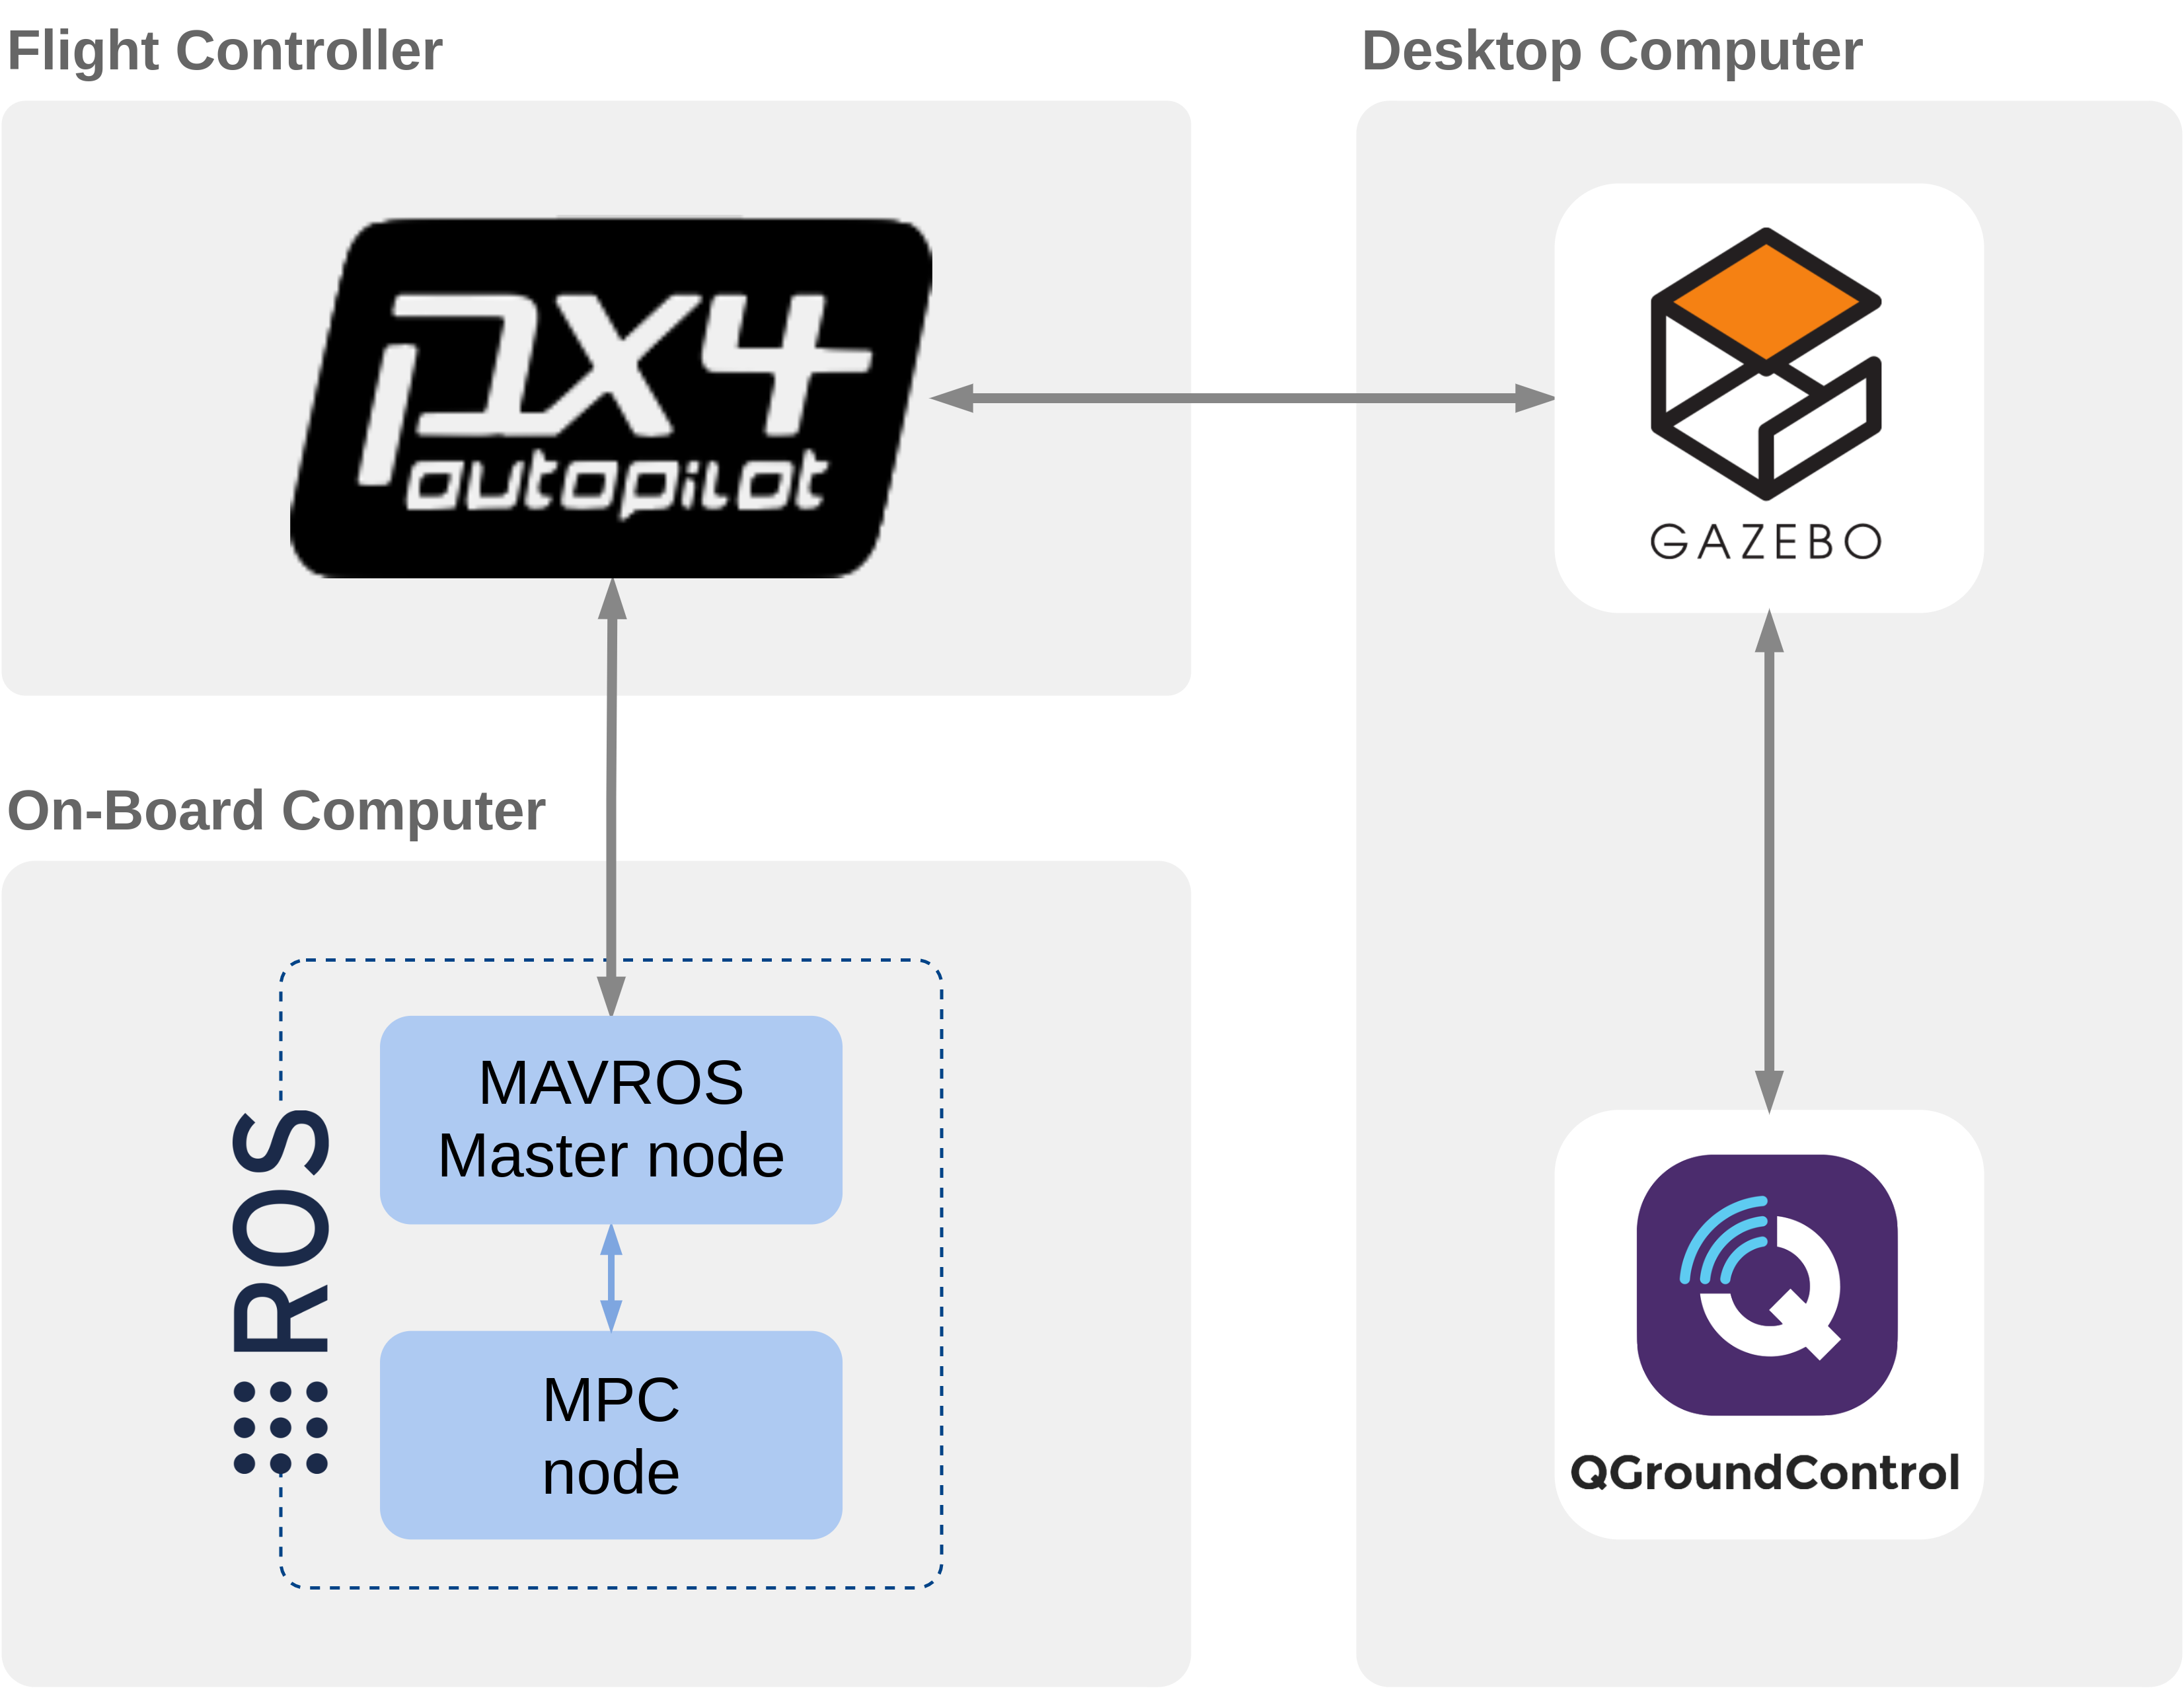
\includegraphics[width=0.8\linewidth]{exp_design/fig/HITL}
            \caption{Different software and hardware components of a \gls{HITL} simulation}
            \label{fig:HITL}
        \end{figure}

    \FloatBarrier\section{Practical flights}

        \paragraph
        The major differences between simulated and practical flights involve wind disturbances and the attachment of the payload.
        In simulations, the payload cable is attached to the exact \gls{CoM} of the multirotor.
        However, for practical flights the cable is attached slightly below the \gls{CoM} of Honeybee due to mechanical constraints.
        Practical flights are also influenced by wind gusts which are difficult to model accurately in simulations.
        The measurement noise experienced by a practical multirotor may also differ from the noise models used in simulations.

        \begin{figure}[!htb]
            \centering
            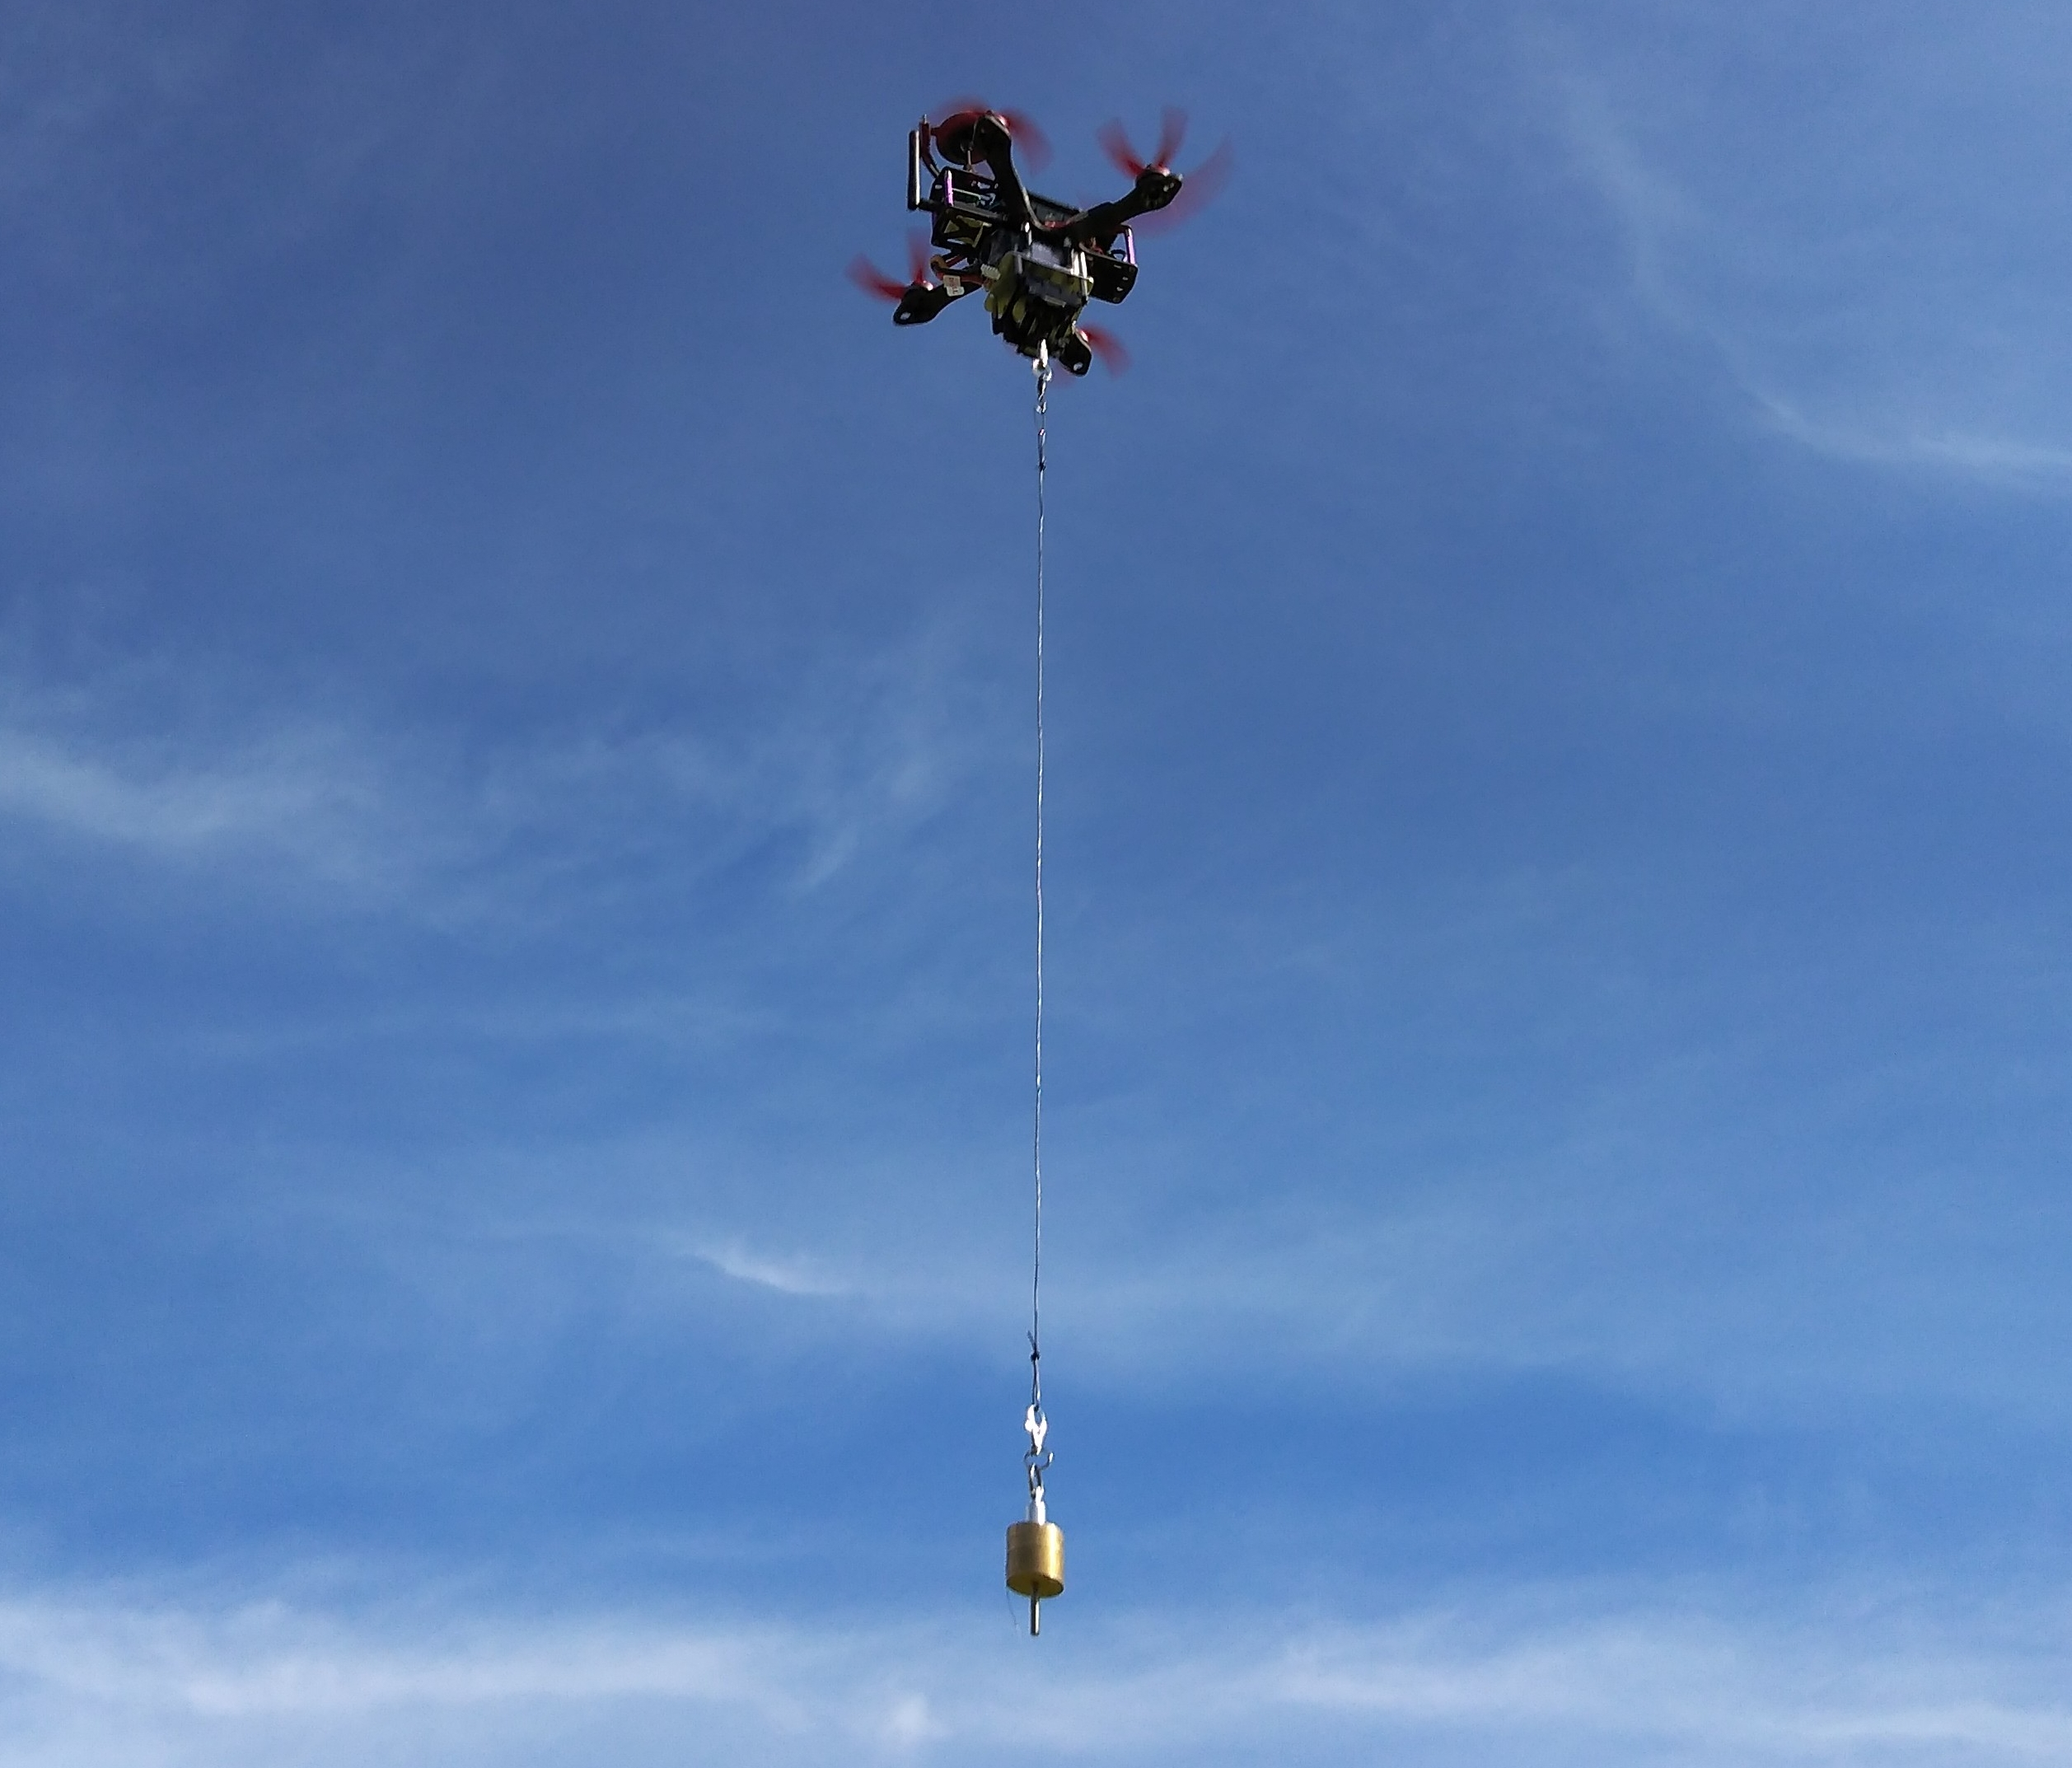
\includegraphics[width=0.7\linewidth]{honeybee_with_payload.jpg}
            \caption{Practical flight with Honeybee and a suspended payload}
            \label{fig:honeybee_with_payload}
        \end{figure}

        \paragraph
        Figure~\ref{fig:honeybee_with_payload} shows Honeybee with a suspended payload during a practical flight.
        Numerous flights were performed with different payload masses, cable lengths and wind conditions.
        Different flights were also performed with a dynamic payload.
        The system identification methods were then applied to the flight data logged by PX4.
        The results of these flight experiments will be discussed in Chapter~\ref{chap:results}.
        
        \paragraph
        % \begin{minipage}{\textwidth} % Use to keep on one page
        The same general methodology used for simulations will be used for practical flights:
        \begin{enumerate}
            \item Arm the multirotor for data logging to start.
            \item Takeoff and hover with the multirotor.
            \item Command velocity step setpoints.
            \item Land the multirotor.
            \item Disarm the multirotor for data logging to stop.
            \item Download the data log from the multirotor.
            \item Split the data into separate training and testing periods.
            \item Build a model from the training data.
            \item Evaluate model predictions with the testing data.
        \end{enumerate}
        % \end{minipage}
        
    \section{Summary}
    
        \paragraph
        This chapter provided an overview of the hardware and software used in this work.
        The \gls{HITL} simulation and practical flight setups were also discussed.
        This provides a background for the experimental tests, results, and discussion in the next chapter.

}
